\title{Nektar++ Tutorial}

\newcommand\gmsh{\emph{Gmsh}~}
\newcommand\nektar{\emph{Nektar++}~}

\documentclass[a4paper,12pt]{article}
\usepackage{tikz}
\usepackage[top=2cm,bottom=3cm,left=1.5cm,right=1.5cm]{geometry}
\usepackage[lined,algo2e,boxed]{algorithm2e}

\setlength{\parindent}{0pt}
\setlength{\parskip}{1ex} 

\begin{document}
\maketitle

The aim of this tutorial is to introduce the user to the spectral/$hp$
element framework \nektar and its use. This guide assumes
the user has successfully compiled the libraries, the solvers and the utilities,
as explained on the website\footnote{www.nektar.info}. A series of regression
tests are included to check that the software is producing the expected results.
Please ensure these all pass before continuing.
\bigskip

In this first section we will create a simple 2D mesh using $Gmsh$ and
convert it into a suitable input format for the \nektar
libraries to process. Subsequently, we will use this mesh to solve a number of
common PDEs already supported by the solvers provided with \nektar, namely:
\begin{enumerate}
\item the Helmholtz equation,
\item the Unsteady Advection-Diffusion equation,
\item the Incompressible Navier-Stokes equations. 
\end{enumerate}

The toy problems discussed initially should aid the user in understanding how to
specify the computational domain (mesh) on which to solve a set of one or more
partial differential equations as well as any necessary parameters, boundary
conditions and initial conditions.

The last step of the tutorial is an example of a more substantial fluid
dynamics problem, the flow past a cylinder. The point of presenting this typical
problem is to introduce some more advanced features including the definition of
curved elements and the use of restart files.


\section{Geometry and Mesh}

We start creating a very simple geometry. A square which we will mesh with 16
quadrilateral elements.
The square is of size
$[-\frac{\pi}{2},\frac{\pi}{2}]\times[-\frac{\pi}{2},\frac{\pi}{2}]$.\\

In the tutorial folder \texttt{NekTutorial/Tutorial/SquareMesh/Geometry/} there
are the following files
\begin{itemize}
\item \texttt{Square.geo} - this is the file containing the geometry
specification defined in terms of \gmsh commands.
\item \texttt{Square.msh} - \gmsh generated mesh data listing mesh vertices and
elements. This is the mesh file understood by the \nektar pre-processing
utilities.
\item \texttt{Square.xml} - \nektar session file generated from
\texttt{Square.msh} using a \nektar utility. This contains only the mesh data at
this stage.
\end{itemize}

If you have \gmsh installed, you can generate the \texttt{.msh} file yourself
from the terminal using the command:

\begin{verbatim}
gmsh -2 Square.geo
\end{verbatim}

or via the graphical user interface. However, we will not discuss the use of
\gmsh in this tutorial. \texttt{Square.xml} has been generated using the
\texttt{MeshConvert} pre-processing tool in the \\
\texttt{utilities/builds/PreProcessing/} directory. To generate the $.xml$ file
from the \texttt{.msh} file, run the command

\begin{verbatim}
./MeshConvert Square.msh Square.xml
\end{verbatim}

Figure \ref{fig:Mesh} shows the resulting mesh on which we are going to
solve a number of PDEs. You can examine the file

\begin{verbatim}
NekTutorial/Tutorial/SquareMesh/Geometry/Square.xml
\end{verbatim}

to see how the various mesh entities have been defined in the \nektar format.

\begin{figure}
\centering
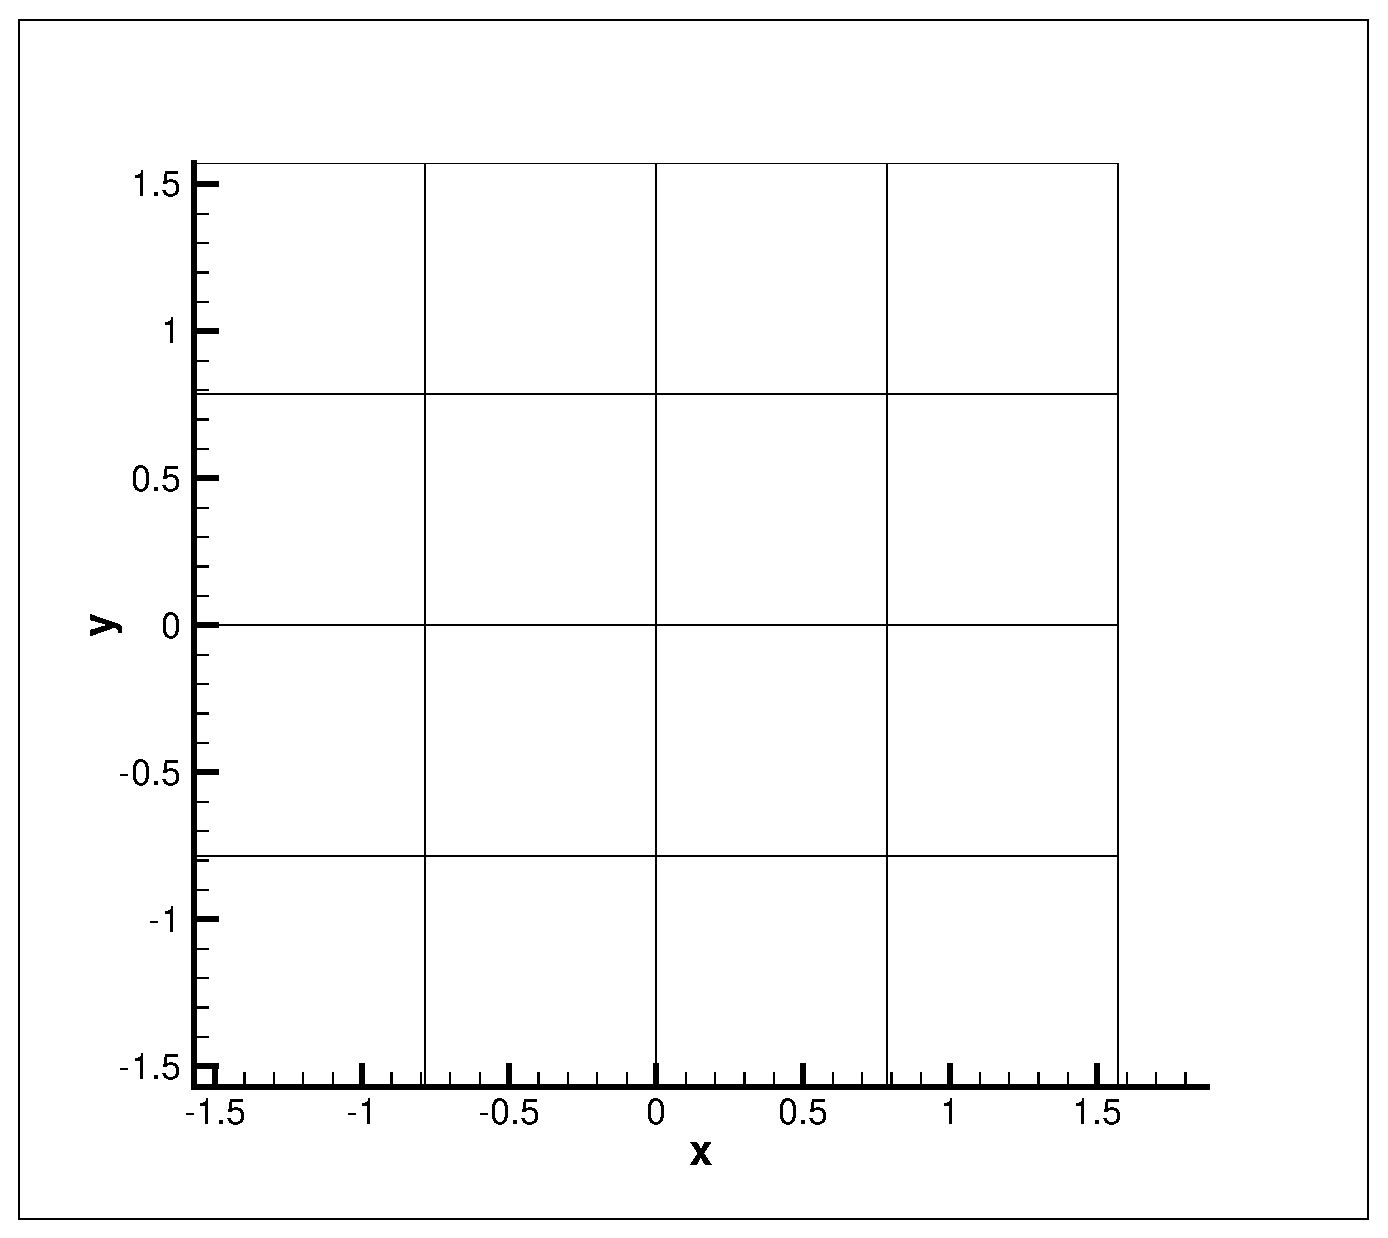
\includegraphics[scale=0.35]{mesh.eps}
\caption{16 quadrilaterals mesh}
\label{fig:Mesh}
\end{figure}


\clearpage
\section{Helmholtz equation}

We begin by solving the 2D Helmholtz equation on the square domain:
\begin{equation}
\nabla^2 u + \lambda u = f \quad u(x,y) \in \Omega
\end{equation}
with smooth forcing function
\begin{equation}
f(x,y)= -(\lambda + 2\pi^2)\sin(\pi x)\sin(\pi y).
\end{equation}
This has the analytic solution
\begin{equation}
u_{ex}(x,y)= \sin(\pi x)\sin(\pi y).
\end{equation}
 
The following files can be found in
\texttt{NekTutorial/Tutorial/SquareMesh/Helmholtz/}:
 \begin{itemize}
 \item \texttt{Test\_HEL.xml} - the \nektar session file containing
 the geometry above and the necessary parameters to solve the Helmholtz problem;
 \item \texttt{Test\_HEL.fld} - solution $u$, obtained using \nektar;
 \item \texttt{Test\_HEL\_u.pos} - post-processed solution $u$ in \gmsh format.
 \end{itemize} 

The \texttt{GEOMETRY} section defines the mesh from the previous section. The
expansion type and order is specified in an \texttt{EXPANSIONS} section. An
expansion basis is applied to a geometry composite specified in the
\texttt{GEOMETRY} section. A default entry is included by \texttt{MeshConvert}.
In this case, \texttt{C[0]} refers to the set of all elements. The \texttt{TYPE}
specifies the choice of polynomial functions to use in the expansion.
Alternatively, for example, one might choose \texttt{FOURIER} or
\texttt{CHEBYSHEV}.

\begin{verbatim}
<EXPANSIONS>
    <E COMPOSITE="C[0]" NUMMODES="8" TYPE="MODIFIED"/>
</EXPANSIONS>
\end{verbatim}

If we examine \texttt{Test\_HEL.xml}, we can see how we can define the
conditions which define the particular problem to solve. These are all enclosed
in a \texttt{CONDITIONS} section.

\begin{enumerate}
\item The equation type, the projection type (\texttt{Continuous} or
\texttt{Discontinuous} Galerkin) and the parameters. Whilst the equation type
and projection type are specified as attributes, the parameters are specified as
name-value pairs. Parameters may be freely used either from within the solver
(e.g. \texttt{Lambda}), or within other expressions, such as function defintions
or other parameters defined subsequently.
\begin{verbatim}
<SOLVERINFO>
    <I PROPERTY="EQTYPE" VALUE="Helmholtz" />
    <I PROPERTY="Projection" VALUE="Continuous" />
</SOLVERINFO>

<PARAMETERS>
    <P> wavefreq       = PI  </P>
    <P> Lambda         = 1.0 </P>
</PARAMETERS>
\end{verbatim}

\item The declaration of the variable(s).  
\begin{verbatim}
<VARIABLES>
    <V ID="0"> u </V> 
</VARIABLES>
\end{verbatim}

\item The specification of boundary regions in terms of composites defined in
the geometry and the conditions applied on those boundaries. The \texttt{REF}
attribute for a boundary condition region should correspond to the \texttt{ID}
of the desired \texttt{BOUNDARYREGION}.
\begin{verbatim}
<BOUNDARYREGIONS>
    <B ID="0"> C[1] </B>
</BOUNDARYREGIONS>

<BOUNDARYCONDITIONS>
    <REGION REF="0">
        <D VAR="u" VALUE="sin(PI*x)*sin(PI*y)">
    </REGION>
</BOUNDARYCONDITIONS>
\end{verbatim}

\item The definition of the forcing term and the exact solution,
\begin{verbatim}
<FORCING>
    <F VAR="u" VALUE="-(Lambda + 2*PI*PI)*sin(PI*x)*sin(PI*y)">
</FORCING>
       
<EXACTSOLUTION>
    <F VAR="u" VALUE="sin(PI*x)*sin(PI*y)">
</EXACTSOLUTION>
\end{verbatim}
\end{enumerate}

This completes the specification of the Helmholtz problem on the square mesh.
It can then be solved using the executable \texttt{ADRSolver}
\footnote{ADRSolver has been design to solve a range of problems in the form of
an Advection-Diffusion-Reaction equation. Switching the EQTYPE flag to
another value and providing the appropriate parameters it can solve, for
example, Poisson, Laplace, Steady/Unsteady Diffusion, Steady/Unsteady Advection,
equations, etc.}. The executable is located in the folder
\texttt{solver/builds/dist/bin/}\footnote{If you compiled the library in Debug
mode, the executables will have the suffix \texttt{-g}.}

\begin{verbatim}
./ADRSolver Test_HEL.xml
\end{verbatim}

To view the output in \gmsh use the post-processing
tools in the \texttt{utilities} directory, as we have done for the
pre-processing. You can produce outputs for \gmsh, $TecPlot$ and $Paraview$
using the corresponding converter from the terminal. For example, to convert the
\texttt{Test\_HEL.fld} to \gmsh format, use

\begin{verbatim}
./FldToGmsh Test_HEL.xml Test_HEL.fld
\end{verbatim} 


\clearpage
\section{Unsteady Advection-Diffusion equation}

Using the same mesh, we will now solve an Unsteady-Advection-Diffusion
problem. As for the Helmholtz problem, the files are located in the directory

\texttt{NekTutorial/Tutorial/SquareMesh/UnsAdvDiffusion/}.

The equation we are solving is
\begin{equation}
\frac{\partial u}{\partial t} + V_X \frac{\partial u}{\partial x} 
    + V_Y \frac{\partial u}{\partial y} = \epsilon \nabla^2 u
\end{equation}

Setting $\epsilon = 1$ and $V_X=V_Y=0$ the exact solution is trivial
and we can use it to set Dirichlet boundary condition on the edges.

\begin{equation}
u_{ex}= e^{-2\pi^2 t}\sin(\pi x)\cos(\pi y)
\end{equation}

In this case the executable is still the \texttt{ADRSolver} but we need to
provide some more information in the input files, including the initial
conditions and the time-integration parameters.

\begin{itemize}
\item Besides changing the \texttt{EQTYPE} to
\texttt{UnsteadyAdvectionDiffusion}, we add a number of additional properties to
specify the approach used in advancing the diffusion and advection components of
the problem. Furthermore, we specify the time-stepping scheme to use.
\begin{verbatim}
<SOLVERINFO>
    <I PROPERTY="EQTYPE" VALUE="UnsteadyAdvectionDiffusion" />
    <I PROPERTY="Projection" VALUE="Continuous" />
    <I PROPERTY="DiffusionAdvancement" VALUE="Implicit" />
    <I PROPERTY="AdvectionAdvancement" VALUE="Explicit" />
    <I PROPERTY="TimeIntegrationMethod" VALUE="IMEXOrder2" />
</SOLVERINFO>
\end{verbatim}

\item Two parameters must be specified for time integration: \texttt{TimeStep}
and \texttt{NumSteps}. The \texttt{IO\_CheckSteps} and \texttt{IO\_InfoSteps}
control the frequency of checkpoint files and status information.
\begin{verbatim}
<PARAMETERS>
    <P> TimeStep       = 0.00001 </P>  
    <P> NumSteps       = 2000    </P>                
    <P> IO_CheckSteps  = 2000    </P>
    <P> IO_InfoSteps   = 2000    </P>
    <P> wavefreq       = PI      </P>                      
    <P> epsilon        = 1.0     </P>
</PARAMETERS>
\end{verbatim}

\item An additional section specifies the advection velocity.
\begin{verbatim}
<USERDEFINEDEQNS>
    <F LHS="Vx" VALUE="0.0" />
    <F LHS="Vy" VALUE="0.0" />
</USERDEFINEDEQNS>
\end{verbatim}

\item Finally, the initial conditions are specified in exactly the same way as
the forcing function and exact solution from the Helmholtz problem.
\begin{verbatim}
<INITIALCONDITIONS>
    <F VAR="u" VALUE="sin(wavefreq*x)*cos(wavefreq*y)" />
</INITIALCONDITIONS>
\end{verbatim}
\end{itemize}

As for the Helmholtz problem, we have included the expected output.


\clearpage
\section{Incompressible Navier-Stokes equations}

Using the same mesh, we can solve the Incompressible Navier-Stokes
equations. In this case the executable in not the \texttt{ADRSolver},
but the \texttt{IncNavierStokesSolver}\footnote{As for the ADRSolver we can have the
Release and the Debug version.}, which is still located in the same
directory as \texttt{ADRSOlver}. All the files, as for the previous examples,
are located in \texttt{NekTutorial/Tutorial/SquareMesh/IncNavStokes/}.

Considering an incompressible, isothermal flow with constant density
and viscosity, the governing equations are the Navier-Stokes (NS) coupled to a
velocity divergence-free constraint. In terms of primitive variables $(V,p)$,
the variational formulation is written as
\begin{equation}
\frac{\partial V}{\partial t} + V \cdot  \nabla V = -\nabla p + \nu \nabla^2 V
\label{eq:NS1}
\end{equation}
\begin{equation}
\nabla \cdot V = 0
\label{eq:NSequation}
\end{equation}
where $p(x,t)$ is the kinematic pressure field and $\nu$ is the kinematic
viscosity. The first flow we are going to solve is the Taylor decaying vortex
described by the following equations

\begin{equation}
u=-\cos(x)\sin(y)e^{-2t/Re}
\label{eq:Dec1}
\end{equation}
\begin{equation}
v=\sin(x)\cos(y)e^{-2t/Re}
\label{eq:Dec2}
\end{equation}
\begin{equation}
p=-\frac{1}{4}\Bigl(\cos(2x)+\cos(2y)\Bigr)e^{-4t/Re}
\label{eq:Dec3}
\end{equation}

In this case we define 3 variables: the 2 velocity components and the pressure.

\begin{verbatim}
<SOLVERINFO>
    <I PROPERTY="EQTYPE" VALUE="UnsteadyNavierStokes" />
    <I PROPERTY="AdvectionForm" VALUE="Convective" />
    <I PROPERTY="TimeIntegrationMethod" VALUE="IMEXOrder1" />
</SOLVERINFO>
\end{verbatim}

\begin{verbatim}
<PARAMETERS>
    <P> TimeStep      = 0.00001 </P>               
    <P> NumSteps      = 1000    </P>                 
    <P> IO_CheckSteps = 1000   </P>                  
    <P> IO_InfoSteps  = 1000   </P>                 
    <P> Kinvis        = 0.0001  </P>            
</PARAMETERS>
\end{verbatim}

\begin{verbatim}
<VARIABLES>
    <V ID="0"> u </V>  
    <V ID="1" v </V>
    <V ID="2" p </V>
</VARIABLES>
\end{verbatim}



\subsection{Flow past a cylinder}
Here a simulation of the two-dimensional flow past a circular cylinder in a free
stream. This is an illustrative example of the use of \nektar framework
to solve more complex fluid dynamics problems The solution, which highlights the
vortex shedding, has been obtained using the $2^{nd}$ order stiffly stable
splitting scheme with $\Delta t = 0.001 s$ and $5^{th}$ order spectral/hp
expansion on a mesh of $1500$ quadrilaterals. The cylinder has a diameter $D =
0.4$ and the domain is defined by a rectangle $[-4\,,16] \times [-5\,,5]$.
Boundary conditions for the velocity filed are of Dirichlet type at the inflow,
where a constant velocity in $x$-direction is imposed ($u = 1$ and $v = 0$) and
of Neumann type (homogeneous) at the outflow and on the upper and lower domain
limits. The pressure boundary conditions are of Neumann type at the inflow and
on the upper and lower domain limits ($\partial p/\partial n = 0$). The pressure
value at the outflow has been set to zero (Dirichlet boundary  condition).\\

In this case the solver is still the \texttt{IncNavierStokesSolver} and all
the files are stored in

\texttt{NekTutorial/Tutorial/VortexShedding/}.

In the
$.xml$ file we can see how curved elements are defined in \nektar and
how we can use a previous solution to initialise the flow. As a matter of fact a
$.rst$ file is actually a $.fld$ file obtained with \nektar and used to
set the flow. In this case we want to start from a converged solution to speed
up the simulation.

\section{Extra examples}

In the folder \texttt{NekTutorial/Tutorial/RegTests/}, you can find plenty of
examples which are directly taken from the regression tests.

\end{document}
